\documentclass[conference]{IEEEtran}
\IEEEoverridecommandlockouts

\usepackage{iftex}
\ifPDFTeX
  \usepackage[T1]{fontenc}
\else
  \usepackage{fontspec}
  \setmainfont{texgyretermes}[Extension=.otf, UprightFont=*-regular,
    BoldFont=*-bold, ItalicFont=*-italic, BoldItalicFont=*-bolditalic]% Times clone for XeLaTeX/Tectonic
\fi
\usepackage{cite}
\usepackage{amsmath,amssymb,amsfonts}
\usepackage{bm}
\usepackage{graphicx}
\usepackage{booktabs}
\usepackage{tabularx}
\usepackage{array}
\usepackage{xcolor}
\usepackage{tikz}
\usetikzlibrary{arrows.meta,positioning,calc,fit}
\usepackage[hidelinks]{hyperref}
\usepackage{url}

\graphicspath{{figures/}}

% ---------------------------------------------------------------- TikZ styles
\definecolor{boxblue}{HTML}{DCE9F7}
\definecolor{boxgreen}{HTML}{DDF1E1}
\definecolor{boxyellow}{HTML}{FFF2CC}
\definecolor{boxpurple}{HTML}{E6E0F5}
\definecolor{edge}{HTML}{2B3A4A}
\tikzset{
  blk/.style={draw=edge, rounded corners=2pt, line width=0.4pt,
              font=\scriptsize, align=center, inner sep=2.5pt,
              minimum height=4.2mm},
  inb/.style={blk, fill=boxblue},
  prc/.style={blk, fill=boxgreen},
  gat/.style={blk, fill=boxyellow},
  llm/.style={blk, fill=boxpurple},
  arr/.style={-{Latex[length=1.6mm,width=1.2mm]}, draw=edge, line width=0.45pt},
}

\begin{document}

\title{Risk-Aware Multi-Agent Decision-Making for Competitive Food Delivery Platforms: Integrating MAPPO, Distributional Reinforcement Learning, Adaptive Risk, LLM/RAG Guidance, and Explainable AI}

\author{
\IEEEauthorblockN{Uday Kiran}
\IEEEauthorblockA{\textit{Department of Artificial Intelligence}\\
\textit{SVNIT Surat}, India\\
i24ai003@aid.svnit.ac.in}
\and
\IEEEauthorblockN{Santhosh}
\IEEEauthorblockA{\textit{Department of Artificial Intelligence}\\
\textit{SVNIT Surat}, India\\
i24ai006@aid.svnit.ac.in}
\and
\IEEEauthorblockN{Rathan}
\IEEEauthorblockA{\textit{Department of Artificial Intelligence}\\
\textit{SVNIT Surat}, India\\
u24ai025@aid.svnit.ac.in}
\and
\IEEEauthorblockN{Samhitha}
\IEEEauthorblockA{\textit{Department of Artificial Intelligence}\\
\textit{SVNIT Surat}, India\\
u24ai080@aid.svnit.ac.in}
\and
\IEEEauthorblockN{Dr.~Nitesh Funde}
\IEEEauthorblockA{\textit{Department of Artificial Intelligence}\\
\textit{SVNIT Surat}, India\\
nitesh.funde@aid.svnit.ac.in}
}

\maketitle

% ================================================================= ABSTRACT
\begin{abstract}
Competitive food delivery platforms operate in dynamic environments characterized by uncertain demand, changing customer preferences, courier-capacity limitations, service delays, and competition between platforms. Effective decision-making in such environments requires balancing profitability, customer fulfilment, operational efficiency, and exposure to adverse outcomes. This research develops a sequential multi-agent decision-making framework for two competing food delivery platforms. The framework progresses through five connected model-building stages. First, a programmable market simulator is established to represent demand, competition, pricing, incentives, courier capacity, customer fulfilment, and operational costs. Second, a Multi-Agent Proximal Policy Optimization (MAPPO) framework is introduced to learn competitive pricing and incentive strategies. Third, distributional reinforcement learning and Conditional Value-at-Risk (CVaR) are incorporated to represent return uncertainty and explicitly account for downside risk. Fourth, adaptive risk estimation is combined with Retrieval-Augmented Generation (RAG), a pretrained instruction-tuned language model, and an uncertainty-gated action prior. This enables contextual guidance while preserving the reinforcement-learning policy as the primary decision-maker. Finally, an Explainable Artificial Intelligence (XAI) framework is developed to investigate decision-level behaviour, feature sensitivity, language-model influence, counterfactual explanations, and explanation faithfulness. The integrated system is evaluated under normal and genuine-shock market conditions. In the reported experiments, the complete Model 4 system improves profit per hour, customer fulfilment, and the reported tail-risk measure relative to its adaptive-risk-only control. The final explainability analysis contains 8,064 decision records across normal and genuine-shock conditions. Feature-faithfulness experiments demonstrate that the highest-ranked features produce substantially larger policy changes than the lowest-ranked features. The results demonstrate a progressive framework that combines competitive multi-agent learning, explicit downside-risk awareness, adaptive contextual guidance, and quantitative explainability.
\end{abstract}

\begin{IEEEkeywords}
Multi-Agent Reinforcement Learning, MAPPO, Food Delivery Platforms, Distributional Reinforcement Learning, Conditional Value-at-Risk, Adaptive Risk, Retrieval-Augmented Generation, Large Language Models, Explainable Artificial Intelligence.
\end{IEEEkeywords}

% ================================================================= 1
\section{Introduction}

\subsection{Background}
Online food delivery platforms operate in competitive markets where multiple platforms serve customers within overlapping geographical and temporal regions. Their operational decisions include pricing, promotional incentives, courier allocation, and service management.

These decisions are interconnected. A pricing change can affect customer demand, while promotional incentives can influence customer selection and order distribution. At the same time, the availability of delivery personnel determines how efficiently incoming orders can be fulfilled.

Consequently, a platform must balance several objectives:
\begin{itemize}
  \item Maximizing operational profitability.
  \item Maintaining high customer fulfilment.
  \item Managing cancellations and unfulfilled orders.
  \item Controlling delivery delays.
  \item Maintaining service-level performance.
  \item Responding to uncertain market conditions.
  \item Considering the strategic behaviour of competing platforms.
\end{itemize}
These characteristics make competitive food delivery an appropriate application domain for multi-agent reinforcement learning.

\subsection{Research Motivation}
Traditional decision-making approaches often optimize individual business objectives independently. However, a competitive delivery platform must make sequential decisions while observing changing market conditions and the actions of competing platforms.

Furthermore, maximizing expected profit alone does not necessarily provide adequate protection against severe negative outcomes. A decision-making system should therefore consider both expected performance and downside risk.

In addition, contextual information can provide useful guidance, but a language model should not automatically replace a learned decision policy. Finally, complex reinforcement-learning policies require methods that can explain why particular decisions were selected.

These motivations lead to a unified framework that combines multi-agent learning, risk-sensitive optimization, contextual language-model guidance, and explainability.

\subsection{Research Objectives}
The principal objectives of this research are:
\begin{enumerate}
  \item Develop a controlled competitive food-delivery market simulator.
  \item Establish a two-agent MAPPO framework for sequential pricing and incentive decisions.
  \item Introduce distributional learning and CVaR-based risk constraints.
  \item Develop an adaptive-risk mechanism that responds to observable market conditions.
  \item Integrate RAG and an instruction-tuned language model through a selective action-prior mechanism.
  \item Develop an XAI framework to measure feature sensitivity, language-model influence, counterfactual behaviour, and explanation faithfulness.
\end{enumerate}

\subsection{Overall Research Contribution}
The research follows five connected model-building stages:
\begin{center}
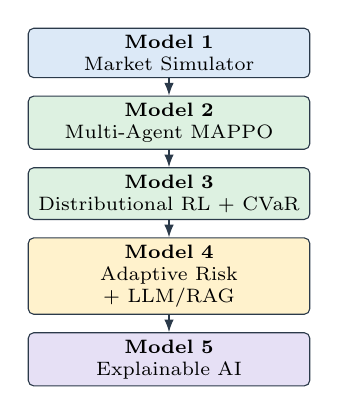
\begin{tikzpicture}[node distance=2.2mm]
  \node[inb, text width=34mm] (m1) {\textbf{Model 1}\\ Market Simulator};
  \node[prc, text width=34mm, below=of m1] (m2) {\textbf{Model 2}\\ Multi-Agent MAPPO};
  \node[prc, text width=34mm, below=of m2] (m3) {\textbf{Model 3}\\ Distributional RL + CVaR};
  \node[gat, text width=34mm, below=of m3] (m4) {\textbf{Model 4}\\ Adaptive Risk + LLM/RAG};
  \node[llm, text width=34mm, below=of m4] (m5) {\textbf{Model 5}\\ Explainable AI};
  \foreach \a/\b in {m1/m2,m2/m3,m3/m4,m4/m5} \draw[arr] (\a) -- (\b);
\end{tikzpicture}
\end{center}
Each stage adds a specific capability to the overall research system. Model 5 operates on the frozen Model 4 policy and provides an explanation and analysis layer rather than another action-selection policy.

% ================================================================= 1b
\section{Related Work}
\emph{Multi-agent RL in mobility markets.} Centralized-critic methods such as MADDPG~\cite{lowe2017maddpg} showed that agents in mixed cooperative--competitive settings can be trained with shared information and executed independently. MAPPO applies the clipped surrogate objective of PPO~\cite{schulman2017ppo}, usually with generalized advantage estimation~\cite{schulman2016gae}, in the same way and is a strong baseline in cooperative tasks~\cite{yu2022mappo}. Closest to our domain, multi-agent RL has been used for large-scale fleet management~\cite{lin2018fleet} and ride-hailing order dispatch~\cite{li2019meanfield}. Those works coordinate vehicles within one platform; we instead model two platforms competing on price and incentives.

\emph{Risk-sensitive RL.} Distributional RL models the whole return distribution rather than its mean~\cite{bellemare2017distributional}, learned in practice with quantile regression~\cite{dabney2018qr} or implicit quantile networks~\cite{dabney2018iqn}. CVaR~\cite{rockafellar2000cvar} is the standard tail-risk measure here. It can be optimized by sampling~\cite{tamar2015cvar} or imposed as a constraint in MDPs~\cite{chow2014cvar}, and Lagrangian methods such as RCPO~\cite{tessler2019rcpo} handle general constraints the same way. Garc\'ia and Fern\'andez survey this wider area of safe RL~\cite{garcia2015safe}. Our Model~3 joins the quantile and constrained-CVaR lines.

\emph{Language models as decision aids.} Retrieval-augmented generation~\cite{lewis2020rag} and instruction-tuned text-to-text models such as T5 and FLAN-T5~\cite{raffel2020t5,chung2024flan} are normally used to generate text. In our system the model only scores candidate actions.

\emph{Explainability.} Local surrogate methods (LIME~\cite{ribeiro2016lime}), Shapley-value attributions (SHAP~\cite{lundberg2017shap}) and integrated gradients~\cite{sundararajan2017ig} assign importance to inputs, and counterfactual explanations~\cite{wachter2018counterfactual} describe the smallest input change that alters a decision. Hooker \emph{et al.}~\cite{hooker2019roar} argued that importance rankings must be checked by perturbing the inputs they rank. We follow that idea: a ranking is only useful if perturbing the top-ranked inputs moves the policy more than perturbing the bottom-ranked ones.

% ================================================================= 2
\section{Datasets and Experimental Environment}

\subsection{Empirical Dataset Sources}
Two publicly available datasets were considered as empirical reference sources for constructing the simulated food-delivery environment.

\subsubsection{Delivery Center: Food and Goods Orders}
The Delivery Center dataset \cite{deliverycenter} contains food and goods delivery order information from Brazil. It provides operational information relevant to understanding delivery-market behaviour. The dataset was used as a reference for characteristics such as:
\begin{itemize}
  \item Temporal order-demand patterns.
  \item Delivery-cycle information.
  \item Operational activity across delivery hubs.
  \item Delivery-related cost characteristics.
  \item Courier and fulfilment-related information.
\end{itemize}

\subsubsection{Zomato Bangalore Restaurants}
The Zomato Bangalore Restaurants dataset \cite{zomato} provides restaurant-level information from the Bangalore market. It was considered as a reference for restaurant-market characteristics, including:
\begin{itemize}
  \item Approximate restaurant pricing.
  \item Restaurant popularity indicators.
  \item Online-ordering characteristics.
  \item Market concentration and restaurant activity.
\end{itemize}

\subsection{Role of the Datasets}
The public datasets served as empirical reference sources for the construction and calibration of the simulated market. The reinforcement-learning agents interacted with the custom simulator rather than directly learning from the raw restaurant and order records. This distinction separates empirical market references from the generated simulation trajectories used for agent training and evaluation.

\subsection{Competitive Market Simulator}
The simulator represents two competing food-delivery platforms, referred to as Agent~A and Agent~B. Each platform observes its market state and selects pricing and incentive decisions. The simulator then processes the combined decisions and generates operational outcomes. The principal environmental components are:
\begin{itemize}
  \item Time-dependent stochastic demand.
  \item Weather-related environmental effects.
  \item Competitor pricing and incentive decisions.
  \item Customer switching behaviour.
  \item Courier availability and operational capacity.
  \item Fulfilled and unfulfilled orders.
  \item Customer cancellations.
  \item Delivery delays and SLA-related outcomes.
  \item Revenue, costs, incentive spending, and profit.
\end{itemize}

\subsection{Market State and Operational Variables}
The simulator maintains information about demand, pricing, incentives, courier capacity, fulfilment, cancellations, delays, and financial outcomes. A simulation step can be represented as:
\begin{equation}
  s_{t+1} = \mathcal{T}\left(s_t, a_t^{A}, a_t^{B}, \xi_t\right),
\end{equation}
where:
\begin{itemize}
  \item $s_t$ is the current market state.
  \item $a_t^{A}$ is the action of Agent~A.
  \item $a_t^{B}$ is the action of Agent~B.
  \item $\xi_t$ represents stochastic environmental effects.
  \item $\mathcal{T}$ is the market transition function.
\end{itemize}
The environment records the operational outcomes generated at every decision step.

\subsection{Observation Representation}
The integrated policy uses a 14-dimensional observation representation. The features describe temporal, environmental, demand, pricing, capacity, service, and operational conditions. The exact semantic mapping is given in Table~\ref{tab:obs}.

\begin{table}[!t]
\centering
\caption{Fourteen-dimensional observation representation.}
\label{tab:obs}
\small
\begin{tabular}{cl}
\toprule
\textbf{Index} & \textbf{Feature} \\
\midrule
0  & Hour sine component \\
1  & Hour cosine component \\
2  & Normalized day index \\
3  & Rain indicator \\
4  & Normalized EWMA demand \\
5  & Normalized own price \\
6  & Normalized own incentive \\
7  & Normalized competitor price \\
8  & Normalized competitor incentive \\
9  & Capacity ratio \\
10 & Fulfilment EWMA \\
11 & Normalized earnings \\
12 & Normalized waiting time \\
13 & Cancellation EWMA \\
\bottomrule
\end{tabular}
\end{table}

\subsection{Action Space}
Each agent selects from a discrete action space combining five pricing levels and five incentive levels. Therefore, the total number of possible actions is:
\begin{equation}
  |\mathcal{A}| = 5 \times 5 = 25.
\end{equation}
An action can be represented as:
\begin{equation}
  a_t = (p_t, w_t),
\end{equation}
where $p_t$ represents the selected pricing level and $w_t$ represents the selected incentive level.

\subsection{Evaluation Episodes}
The simulator supports repeatable evaluation episodes of 168 decision steps. This enables the collection of sequential operational outcomes and policy decisions under controlled environmental conditions.

% ================================================================= 3
\section{Model 1: Basic Market and Delivery Simulator}

\subsection{Objective}
Model 1 establishes the operational foundation of the research system. Its purpose is to create a programmable environment in which two competing delivery platforms can interact through sequential decisions.

\subsection{Architecture}
The architecture of the simulator is shown in Fig.~\ref{fig:m1arch}.

\begin{figure}[!t]
\centering
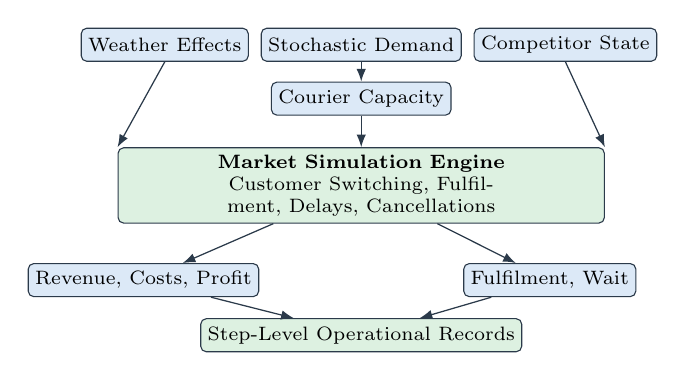
\begin{tikzpicture}[node distance=3mm and 1.5mm]
  \node[inb] (dem) {Stochastic Demand};
  \node[inb, left=of dem] (wea) {Weather Effects};
  \node[inb, right=of dem] (cmp) {Competitor State};
  \node[inb, below=2.5mm of dem] (cap) {Courier Capacity};
  \node[prc, below=4mm of cap, text width=60mm] (eng)
       {\textbf{Market Simulation Engine}\\ Customer Switching, Fulfilment, Delays, Cancellations};
  \node[inb, below left=5mm and -18mm of eng] (rev) {Revenue, Costs, Profit};
  \node[inb, below right=5mm and -18mm of eng] (ful) {Fulfilment, Wait};
  \node[prc, below=12mm of eng] (rec) {Step-Level Operational Records};
  \draw[arr] (wea.south) -- (eng.north west);
  \draw[arr] (cmp.south) -- (eng.north east);
  \draw[arr] (dem) -- (cap);
  \draw[arr] (cap) -- (eng);
  \draw[arr] (eng) -- (rev);
  \draw[arr] (eng) -- (ful);
  \draw[arr] (rev) -- (rec);
  \draw[arr] (ful) -- (rec);
\end{tikzpicture}
\caption{Architecture of Model 1: Competitive market simulator.}
\label{fig:m1arch}
\end{figure}

\subsection{Core Functionalities}
The simulator incorporates the following mechanisms:
\begin{enumerate}
  \item Stochastic and time-dependent demand generation.
  \item Weather-related demand effects.
  \item Competitor pricing and incentive interactions.
  \item Customer switching between platforms.
  \item Courier availability and capacity constraints.
  \item Order fulfilment and cancellation mechanisms.
  \item Delivery delay and service-level calculations.
  \item Revenue, operational cost, and profit accounting.
  \item Detailed step-level logging.
\end{enumerate}

\subsection{Operational Performance Measurements}
The simulator records the following outcomes:
\begin{itemize}
  \item Profit and revenue.
  \item Fulfilled and unfulfilled orders.
  \item Customer cancellations.
  \item Delivery delays.
  \item Incentive spending.
  \item Routine delay costs.
  \item Service-level outcomes.
\end{itemize}

\subsection{Model 1 Outcome}
Model 1 successfully established a repeatable competitive market environment. The same environment subsequently supported multi-agent policy training, risk-sensitive optimization, controlled market-shock experiments, and decision-level explainability analysis. This provided a common experimental foundation for all subsequent models.

% ================================================================= 4
\section{Model 2: Competitive Multi-Agent MAPPO}

\subsection{Objective}
Model 2 introduces learning-based decision-making into the simulated market. Instead of relying on manually specified pricing and incentive rules, two agents learn policies through interaction with the shared environment. The selected reinforcement-learning approach is Multi-Agent Proximal Policy Optimization (MAPPO) \cite{schulman2017ppo,yu2022mappo}.

\subsection{MAPPO Framework}
MAPPO extends PPO-style policy optimization to multi-agent environments. Each platform maintains its own policy actor, while learning is performed using state and reward information from the shared environment. The framework follows the centralized-training and decentralized-execution principle.

\subsection{Model Architecture}
The two-agent architecture is shown in Fig.~\ref{fig:m2arch}.

\begin{figure}[!t]
\centering
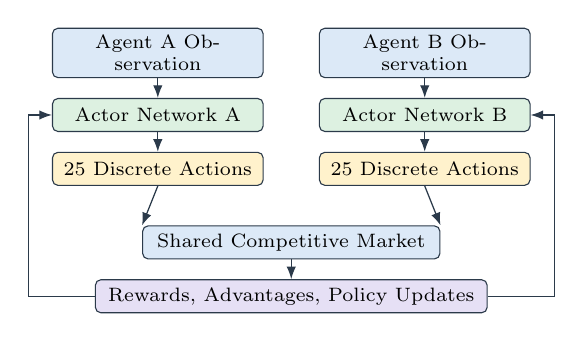
\begin{tikzpicture}[node distance=2.5mm]
  \node[inb, text width=25mm] (oa) {Agent A Observation};
  \node[prc, text width=25mm, below=of oa] (na) {Actor Network A};
  \node[gat, text width=25mm, below=of na] (da) {25 Discrete Actions};
  \node[inb, text width=25mm, right=7mm of oa] (ob) {Agent B Observation};
  \node[prc, text width=25mm, below=of ob] (nb) {Actor Network B};
  \node[gat, text width=25mm, below=of nb] (db) {25 Discrete Actions};
  \path (da.south) -- (db.south) coordinate[midway] (mid);
  \node[inb, text width=36mm, below=5mm of mid] (mk) {Shared Competitive Market};
  \node[llm, text width=48mm, below=of mk] (up) {Rewards, Advantages, Policy Updates};
  \draw[arr] (oa) -- (na); \draw[arr] (na) -- (da);
  \draw[arr] (ob) -- (nb); \draw[arr] (nb) -- (db);
  \draw[arr] (da.south) -- (mk.north west);
  \draw[arr] (db.south) -- (mk.north east);
  \draw[arr] (mk) -- (up);
  \draw[arr] (up.west) -| ([xshift=-3mm]na.west) -- (na.west);
  \draw[arr] (up.east) -| ([xshift=3mm]nb.east) -- (nb.east);
\end{tikzpicture}
\caption{Two-agent MAPPO architecture.}
\label{fig:m2arch}
\end{figure}

\subsection{Actor Network}
Each actor receives a 14-dimensional observation and produces a categorical probability distribution over the 25 available actions. The actor architecture is:
\begin{equation}
  14 \rightarrow 128 \rightarrow 128 \rightarrow 25.
\end{equation}
The network uses two hidden layers with 128 units and hyperbolic tangent activation functions. The output represents the action logits used to construct a categorical policy distribution.

\subsection{Policy Optimization}
The PPO clipped objective \cite{schulman2017ppo} is:
\begin{equation}
  L^{CLIP}(\theta) = \mathbb{E}_t\!\left[\min\!\left(r_t(\theta)\hat{A}_t,\,
  \mathrm{clip}\!\left(r_t(\theta),1-\epsilon,1+\epsilon\right)\hat{A}_t\right)\right],
\end{equation}
where:
\begin{equation}
  r_t(\theta) = \frac{\pi_\theta(a_t \mid o_t)}{\pi_{\theta_{\mathrm{old}}}(a_t \mid o_t)}.
\end{equation}
Here, $\hat{A}_t$ represents the estimated advantage and $\epsilon$ controls the policy update clipping range.

\subsection{Training and Learning Process}
The two agents interact with the shared market, observe their individual market states, select pricing and incentive actions, and receive rewards based on the resulting market outcomes. The collected trajectories are used to update the actor and value-learning components.

\subsection{Model 2 Outcome}
Model 2 established a trainable competitive two-agent MAPPO baseline. The model produced reusable policy checkpoints that provided the initialization foundation for the subsequent risk-sensitive learning stage. It also established the 14-dimensional observation representation and 25-action decision structure used by later models.

% ================================================================= 5
\section{Model 3: Distributional and CVaR-Constrained MAPPO}

\subsection{Motivation}
Expected return alone does not describe the complete performance distribution of a policy. Two policies may have similar average returns while exhibiting different levels of downside risk. Model 3 introduces distributional reinforcement learning \cite{bellemare2017distributional} and CVaR-based optimization \cite{rockafellar2000cvar} to represent and control adverse outcomes.

\subsection{Distributional Critic}
The distributional critic predicts multiple quantiles of the return distribution rather than estimating only a single expected value. The implemented critic predicts
\begin{equation}
  N_q = 25
\end{equation}
quantiles. The predicted quantile values are:
\begin{equation}
  Z(s) = \{z_1(s), z_2(s), \ldots, z_{25}(s)\}.
\end{equation}
Quantile regression provides a learning mechanism for approximating the return distribution \cite{dabney2018qr}.

\subsection{Quantile Huber Loss}
The quantile regression objective is based on the quantile Huber loss:
\begin{equation}
  L_\kappa = \frac{1}{N_q}\sum_{i=1}^{N_q}\left|\tau_i - \mathbb{I}(\delta_i < 0)\right| \mathcal{L}_\kappa(\delta_i),
\end{equation}
where $\delta_i$ is the temporal-difference error associated with quantile $i$.

\subsection{Conditional Value-at-Risk}
Conditional Value-at-Risk measures the expected severity of outcomes in a selected tail of the return or loss distribution. The project uses:
\begin{equation}
  \alpha = 0.10.
\end{equation}
This corresponds to a 10\% tail level. The risk-sensitive objective considers the lower-tail performance of the policy.

\subsection{Primal-Dual Risk Constraint}
A primal-dual mechanism is introduced to penalize violations of the specified risk limit \cite{chow2014cvar}. The constrained objective can be expressed conceptually as:
\begin{equation}
  \max_{\pi}\; J(\pi) \quad \text{subject to} \quad \mathrm{CVaR}_\alpha(\pi) \le C,
\end{equation}
where $C$ represents the specified risk limit. The corresponding Lagrangian formulation is:
\begin{equation}
  \mathcal{L}(\pi,\lambda) = J(\pi) - \lambda\left(\mathrm{CVaR}_\alpha(\pi) - C\right).
\end{equation}
The multiplier $\lambda$ is updated through the primal-dual optimization procedure.

\subsection{Model 3 Architecture}
The distributional and CVaR-constrained learning architecture is shown in Fig.~\ref{fig:m3arch}.

\begin{figure}[!t]
\centering
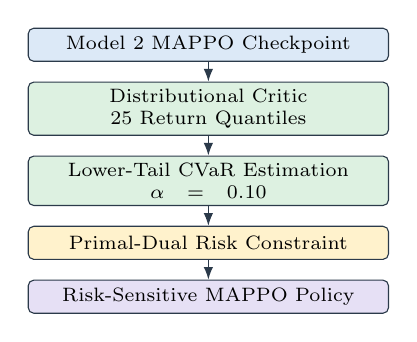
\begin{tikzpicture}[node distance=2.5mm]
  \node[inb, text width=44mm] (c) {Model 2 MAPPO Checkpoint};
  \node[prc, text width=44mm, below=of c] (d) {Distributional Critic\\ 25 Return Quantiles};
  \node[prc, text width=44mm, below=of d] (v) {Lower-Tail CVaR Estimation\\ $\alpha = 0.10$};
  \node[gat, text width=44mm, below=of v] (p) {Primal-Dual Risk Constraint};
  \node[llm, text width=44mm, below=of p] (r) {Risk-Sensitive MAPPO Policy};
  \foreach \a/\b in {c/d,d/v,v/p,p/r} \draw[arr] (\a) -- (\b);
\end{tikzpicture}
\caption{Distributional and CVaR-constrained learning architecture.}
\label{fig:m3arch}
\end{figure}

\subsection{Reported Evaluation Findings}
The reported earlier evaluation demonstrates improvements in customer fulfilment and the downside-risk measure (Table~\ref{tab:m3}).

\begin{table}[!t]
\centering
\caption{Reported Model 3 fulfilment and tail-risk findings.}
\label{tab:m3}
\small
\begin{tabular}{lccc}
\toprule
\textbf{Metric} & \textbf{Model 2} & \textbf{Model 3} & \textbf{Change} \\
\midrule
Fulfilment rate & 0.852 & 0.867 & +1.5 pp \\
Tail CVaR       & 4.545 & 4.111 & 9.55\% reduction \\
\bottomrule
\end{tabular}
\end{table}

\subsection{Model 3 Outcome}
Model 3 established explicit downside-risk awareness within the multi-agent learning system. The distributional critic represented return uncertainty through 25 quantiles, while CVaR and primal-dual optimization incorporated risk constraints into policy learning. The reported evaluation showed improved fulfilment and a lower tail-risk measure.

% ================================================================= 6
\section{Model 4: Adaptive Risk and Uncertainty-Gated LLM/RAG Guidance}

\subsection{Objective}
Model 4 extends the risk-sensitive MAPPO framework by introducing adaptive risk estimation and contextual guidance from an LLM. The central design principle is that the reinforcement-learning policy remains responsible for the final action. The LLM provides an additional action prior, whose influence is controlled by a confidence gate.

\subsection{Adaptive Risk Estimation}
A risk estimator processes observable market conditions and historical information to estimate the current level of market risk. The estimator uses observable information rather than directly accessing a hidden future shock label. The adaptive risk coefficient is mapped to a bounded range:
\begin{equation}
  \lambda_t = 0.10 + r_t(0.60 - 0.10),
\end{equation}
where $r_t$ is the estimated risk score. Thus:
\begin{equation}
  0.10 \le \lambda_t \le 0.60.
\end{equation}
This allows the system to adjust its risk sensitivity according to observed conditions.

\subsection{Validation of Stress Sensitivity}
The adaptive-risk estimator was evaluated under normal and genuine-shock conditions. The observed mean risk scores are listed in Table~\ref{tab:risk}.

\begin{table}[!t]
\centering
\caption{Adaptive risk under normal and genuine-shock conditions.}
\label{tab:risk}
\small
\begin{tabular}{lc}
\toprule
\textbf{Condition} & \textbf{Mean Risk Score} \\
\midrule
Normal market        & 0.4072 \\
Genuine-shock market & 0.7019 \\
\bottomrule
\end{tabular}
\end{table}

The higher risk score under genuine shock demonstrates that the estimator responds to increased environmental stress. Fig.~\ref{fig:risk} plots the same means together with the standard deviation of the per-decision risk score in each condition (0.0608 for normal and 0.1208 for genuine shock, 4,032 decision records each). The spread of the score is also wider under genuine shock.

\begin{figure}[!t]
\centering
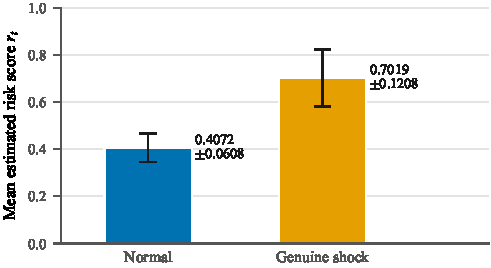
\includegraphics[width=\columnwidth]{fig_risk_estimator}
\caption{Response of the adaptive risk estimator. Bars give the mean estimated risk score $r_t$ over 4,032 decision records per condition; error bars give $\pm 1$ standard deviation of the per-decision score (not a confidence interval).}
\label{fig:risk}
\end{figure}

\subsection{Retrieval-Augmented Generation}
RAG \cite{lewis2020rag} provides relevant contextual information to the language-model component. The retrieval mechanism supplies contextual material that can support the generation or scoring of candidate decision guidance. The LLM component used in Model 4 is Google's pretrained FLAN-T5-Small model \cite{chung2024flan,flant5small}. The model was used as a contextual guidance component rather than as an independent market controller.

\subsection{Contrastive Action-Prior Generation}
The initial structured-generation approach was replaced with a contrastive likelihood mechanism. The action space contains five price levels and five incentive levels. For each candidate price and incentive combination, the language model provides likelihood-based scores. These scores are converted into a probability distribution over the 25 candidate actions. The resulting distribution is denoted by:
\begin{equation}
  P_{\mathrm{LLM}}(a \mid s).
\end{equation}
This mechanism produces a structured action prior without requiring the language model to directly control the environment.

\subsection{Uncertainty Gate}
The LLM action prior is integrated with the reinforcement-learning policy through a confidence gate. The gate controls the influence of the LLM-generated prior on the actor logits. A conceptual representation is:
\begin{equation}
  \ell_{\mathrm{combined}} = \ell_{\mathrm{RL}} + g_t \log\left(P_{\mathrm{LLM}}(a \mid s) + \varepsilon\right),
\end{equation}
where:
\begin{itemize}
  \item $\ell_{\mathrm{RL}}$ represents MAPPO actor logits.
  \item $P_{\mathrm{LLM}}$ represents the LLM action prior.
  \item $g_t$ represents the confidence gate.
  \item $\varepsilon$ provides numerical stability.
\end{itemize}
The combined logits are used to construct the final categorical policy. This preserves MAPPO as the primary decision-making mechanism.

\subsection{Model 4 Architecture}
The integration of the adaptive-risk and LLM/RAG components is shown in Fig.~\ref{fig:m4arch}.

\begin{figure}[!t]
\centering
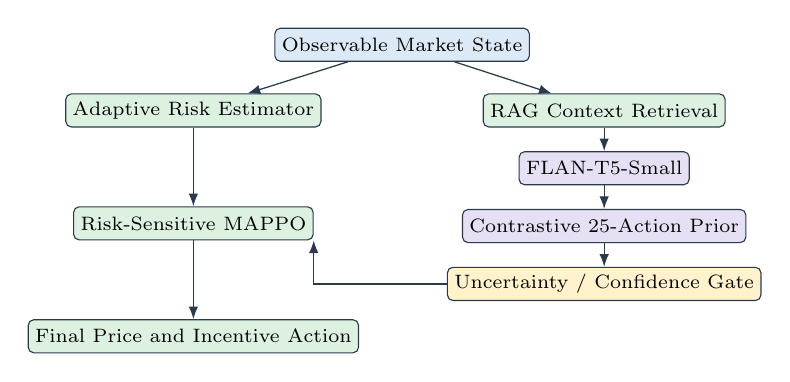
\begin{tikzpicture}[node distance=3mm and 2mm]
  \node[inb] (st) {Observable Market State};
  \node[prc, below left=4mm and -6mm of st] (re) {Adaptive Risk Estimator};
  \node[prc, below right=4mm and -6mm of st] (rg) {RAG Context Retrieval};
  \node[llm, below=of rg] (ft) {FLAN-T5-Small};
  \node[llm, below=of ft] (pr) {Contrastive 25-Action Prior};
  \node[gat, below=of pr] (gt) {Uncertainty / Confidence Gate};
  \node[prc, below=10mm of re] (mp) {Risk-Sensitive MAPPO};
  \node[prc, below=10mm of mp] (fa) {Final Price and Incentive Action};
  \draw[arr] (st) -- (re); \draw[arr] (st) -- (rg);
  \draw[arr] (rg) -- (ft); \draw[arr] (ft) -- (pr); \draw[arr] (pr) -- (gt);
  \draw[arr] (re) -- (mp);
  \draw[arr] (gt.west) -| (mp.south east);
  \draw[arr] (mp) -- (fa);
\end{tikzpicture}
\caption{Model 4: Adaptive-risk and uncertainty-gated LLM/RAG integration.}
\label{fig:m4arch}
\end{figure}

\subsection{Training Configuration}
The complete integrated Model 4 policy was trained for 1,500 updates. The adaptive-risk-only control was trained for 1,000 updates. The integrated training configuration included the distributional and risk-sensitive components inherited from the preceding risk-sensitive framework. The training record reported:
\begin{itemize}
  \item 1,500 completed integrated training updates.
  \item 1,000 adaptive-risk control updates.
  \item 3,000 successful LLM prior calls.
  \item Zero recorded parsing failures.
\end{itemize}

\subsection{Normal-Condition Evaluation}
The complete Model 4 system was compared against its adaptive-risk-only control under normal market conditions (Table~\ref{tab:m4normal}).

\begin{table}[!t]
\centering
\caption{Model 4 normal-condition results.}
\label{tab:m4normal}
\small
\setlength{\tabcolsep}{4pt}
\begin{tabular}{lccc}
\toprule
\textbf{Metric} & \textbf{Adaptive} & \textbf{Full} & \textbf{Improvement} \\
 & \textbf{Control} & \textbf{Model 4} & \\
\midrule
Profit per hour & 344.8984 & 356.0009 & 3.22\% increase \\
Fulfilment rate & 0.8504   & 0.8775   & 2.71 pp \\
Tail CVaR       & 4.8128   & 4.2483   & 11.75\% reduction \\
\bottomrule
\end{tabular}
\end{table}

The integrated system achieved higher profitability and fulfilment while also reducing the reported tail-risk measure.

\subsection{Genuine-Shock Evaluation}
The same comparison was performed under genuine-shock market conditions (Table~\ref{tab:m4shock}).

\begin{table}[!t]
\centering
\caption{Model 4 genuine-shock results.}
\label{tab:m4shock}
\small
\setlength{\tabcolsep}{4pt}
\begin{tabular}{lccc}
\toprule
\textbf{Metric} & \textbf{Adaptive} & \textbf{Full} & \textbf{Improvement} \\
 & \textbf{Control} & \textbf{Model 4} & \\
\midrule
Profit per hour & 314.2400 & 328.2573 & 4.46\% increase \\
Fulfilment rate & 0.8124   & 0.8424   & 3.00 pp \\
Tail CVaR       & 5.3776   & 4.8655   & 9.53\% reduction \\
\bottomrule
\end{tabular}
\end{table}

The integrated policy maintained improvements in profitability and fulfilment while reducing the reported downside-risk measure under genuine environmental stress.

\subsection{Model 4 Outcome}
Model 4 successfully integrated adaptive risk estimation, distributional risk-sensitive learning, RAG-based contextual information, FLAN-T5-Small, and an uncertainty-gated action prior. The final action continued to be selected by the MAPPO policy. Across both tested conditions, the full integrated system improved all three reported evaluation outcomes relative to the adaptive-risk-only control. Fig.~\ref{fig:m4perf} places the values of Tables~\ref{tab:m4normal} and~\ref{tab:m4shock} side by side; each metric is drawn on its own axis because the three measures have different units.

\begin{figure*}[!t]
\centering
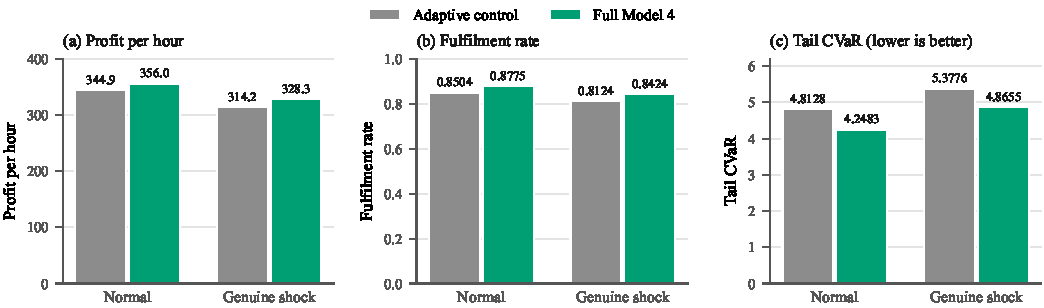
\includegraphics[width=\textwidth]{fig_model4_performance}
\caption{Model 4 performance comparison between the adaptive-risk-only control and the full Model 4 system under normal and genuine-shock conditions: (a) profit per hour, (b) fulfilment rate, and (c) tail CVaR, where a lower value indicates a smaller downside risk. Values are taken from Tables~\ref{tab:m4normal} and~\ref{tab:m4shock}.}
\label{fig:m4perf}
\end{figure*}

\subsection{Shock-Condition Validation}
The genuine-shock setting raises the demand volatility parameter of the simulator from $\sigma_\lambda = 0.12$ in the normal setting to $\sigma_\lambda = 0.30$. To check that this change is present in the evaluated episodes, the demand noise was recovered from 672 simulation steps in each condition. The recovered standard deviation was 0.1193 under normal conditions and 0.2940 under genuine shock, a ratio of 2.46 against the configured ratio of 2.50. The mean absolute noise rose from 0.0960 to 0.2365, and the 95th percentile of the absolute noise rose from 0.2344 to 0.5685. These values are compared in Fig.~\ref{fig:shock}.

\begin{figure}[!t]
\centering
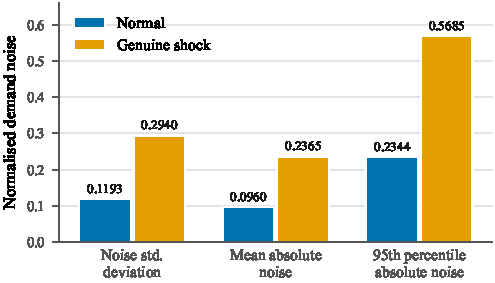
\includegraphics[width=\columnwidth]{fig_shock_validation}
\caption{Shock-condition validation: standard deviation, mean absolute value, and 95th percentile absolute value of the recovered normalised demand noise, computed from 672 simulation steps in each condition.}
\label{fig:shock}
\end{figure}

% ================================================================= 7
\section{Model 5: Explainable AI for the Integrated Decision System}

\subsection{Objective}
Model 5 introduces an explainability layer for the frozen Model 4 policy. Unlike the previous models, Model 5 does not train a new action-selection policy. Instead, it investigates how the integrated policy makes decisions and whether the identified important features correspond to actual policy behaviour. The principal components are:
\begin{itemize}
  \item Decision-level logging.
  \item Semantic observation mapping.
  \item Integrated-policy feature sensitivity.
  \item LLM influence analysis.
  \item Counterfactual explanations.
  \item Explanation-faithfulness evaluation.
\end{itemize}

\subsection{Decision-Level Logging}
The logging system records information associated with each policy decision. The recorded information includes:
\begin{itemize}
  \item Observation vectors.
  \item Action probabilities.
  \item Selected actions.
  \item Adaptive risk scores.
  \item LLM action priors.
  \item Confidence-gate values.
  \item Simulator state and operational outcomes.
\end{itemize}
The initial pilot validated the logging pipeline with 672 decision records across two episodes. The complete normal and genuine-shock analyses subsequently produced:
\begin{equation}
  N_{\mathrm{total}} = 4032 + 4032 = 8064.
\end{equation}

\subsection{Integrated-Policy Feature Sensitivity}
Feature sensitivity analysis investigates how changes in individual observation features affect the policy's action preferences. The frozen policy is evaluated under controlled feature perturbations. The analysis considers changes in:
\begin{itemize}
  \item Selected-action preference.
  \item Action-logit margins.
  \item Predicted action probabilities.
  \item Action-selection stability.
\end{itemize}
This allows the importance of each observation feature to be examined through its influence on the integrated decision policy.

\subsection{Feature Ranking}
The feature-sensitivity analysis identifies the following leading features:
\begin{enumerate}
  \item Hour sine component.
  \item Hour cosine component.
  \item Normalized EWMA demand.
  \item Normalized waiting time.
  \item Normalized competitor price.
  \item Normalized own price.
  \item Capacity ratio.
\end{enumerate}
These features represent temporal market conditions, demand, customer waiting conditions, competitive pricing, and operational capacity.

\subsection{LLM Influence Analysis}
The LLM influence analysis measures the difference between decisions made with and without the LLM action prior. The analysis records:
\begin{itemize}
  \item Mean confidence-gate value.
  \item Action-change rate.
  \item Policy divergence.
  \item Logit changes.
\end{itemize}
The results demonstrate selective LLM influence rather than unrestricted replacement of the reinforcement-learning policy (Table~\ref{tab:llm}).

\begin{table}[!t]
\centering
\caption{LLM influence under normal and genuine-shock conditions.}
\label{tab:llm}
\small
\begin{tabular}{lcc}
\toprule
\textbf{Metric} & \textbf{Normal} & \textbf{Genuine Shock} \\
\midrule
Mean confidence gate & 0.1340 & 0.1322 \\
Action-change rate   & 1.54\% & 1.84\% \\
Mean adaptive risk   & 0.4072 & 0.7019 \\
\bottomrule
\end{tabular}
\end{table}

\subsection{Counterfactual Explanations}
Counterfactual analysis investigates whether realistic changes in individual observation features can alter the selected policy action. For each sampled decision, the analysis perturbs selected input features while holding the recorded LLM prior and confidence-gate values fixed. This isolates the effect of observation changes on the policy's action selection. The resulting explanations identify feature modifications associated with actual changes in the selected action.

\subsection{Explanation Faithfulness}
An important requirement of an explanation method is that its feature ranking should reflect the actual behaviour of the underlying policy. The project evaluates this through a comparison between high-ranked and low-ranked features. Two measurements are considered:
\begin{enumerate}
  \item Action-flip ratio.
  \item Decision-margin-change ratio.
\end{enumerate}
The action-flip ratio compares the action changes caused by perturbing top-ranked features against those caused by perturbing bottom-ranked features. The margin-change ratio performs a similar comparison using policy decision margins.

\subsection{Model 5 Quantitative Results}
The final XAI analysis produced the results in Table~\ref{tab:xai}.

\begin{table}[!t]
\centering
\caption{Model 5 explainability results.}
\label{tab:xai}
\small
\setlength{\tabcolsep}{4pt}
\begin{tabular}{lcc}
\toprule
\textbf{Measurement} & \textbf{Normal} & \textbf{Genuine Shock} \\
\midrule
Decision records                 & 4,032          & 4,032 \\
Mean adaptive risk               & 0.4072         & 0.7019 \\
Mean LLM gate                    & 0.1340         & 0.1322 \\
LLM action-change rate           & 1.54\%         & 1.84\% \\
Top/bottom action-flip ratio     & 7.38$\times$   & 8.86$\times$ \\
Top/bottom margin ratio          & 20.33$\times$  & 21.21$\times$ \\
Counterfactual decision coverage & 36.33\%        & 35.94\% \\
\bottomrule
\end{tabular}
\end{table}

The ratios in Table~\ref{tab:xai} are formed from the underlying flip rates and margin changes shown in Fig.~\ref{fig:faith}, each measured on 256 perturbed samples per group. Under normal conditions, perturbing the top-ranked features flipped 23.0\% of actions against 3.1\% for the bottom-ranked features, with mean absolute margin changes of 1.407 and 0.069. Under genuine shock, the corresponding values were 24.2\% against 2.7\% and 1.455 against 0.069.

\begin{figure}[!t]
\centering
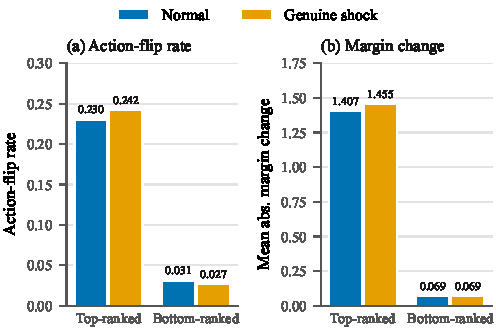
\includegraphics[width=\columnwidth]{fig_faithfulness}
\caption{Explanation faithfulness: (a) action-flip rate and (b) mean absolute action-margin change when the top-ranked and bottom-ranked features are perturbed, under normal and genuine-shock conditions (256 samples per group).}
\label{fig:faith}
\end{figure}

Fig.~\ref{fig:llmcf}(a) shows the LLM influence measures of Table~\ref{tab:llm} together with the mean KL divergence between the full and RL-only policies ($1.906\times10^{-4}$ normal, $1.785\times10^{-4}$ genuine shock) and the mean absolute logit change (0.5085 and 0.5000). Fig.~\ref{fig:llmcf}(b) summarises the counterfactual search: 363 and 364 successful counterfactuals were found, covering 36.33\% and 35.94\% of the sampled decisions, with feature-level flip rates of 10.13\% and 10.16\%.

\begin{figure*}[!t]
\centering
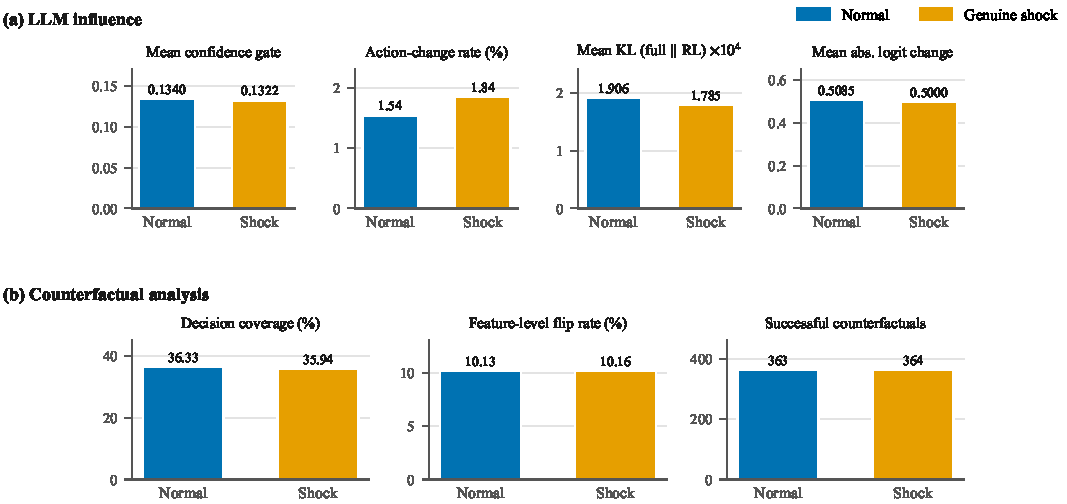
\includegraphics[width=\textwidth]{fig_llm_counterfactual}
\caption{LLM influence and counterfactual analysis under normal and genuine-shock conditions. (a) LLM influence: mean confidence gate, action-change rate, mean KL divergence between the full and RL-only policies, and mean absolute logit change. (b) Counterfactual analysis: unique decision coverage, feature-level flip rate, and number of successful counterfactuals. Each panel uses its own axis because the metrics differ in scale and unit.}
\label{fig:llmcf}
\end{figure*}

\subsection{Model 5 Outcome}
Model 5 successfully established a quantitative explainability framework for the frozen integrated policy. The analysis identified the most influential observation features, measured the influence of the LLM, and evaluated whether feature rankings corresponded to actual policy sensitivity \cite{sundararajan2017ig}. The top-ranked features produced substantially larger action changes and decision-margin changes than the bottom-ranked features. The counterfactual experiments also demonstrated that controlled changes to operational observations can produce different policy decisions.

% ================================================================= 8
\section{Integrated Research System}

\subsection{Complete Architecture}
The five models form a connected decision-making and analysis pipeline, shown in Fig.~\ref{fig:full}.

\begin{figure}[!t]
\centering
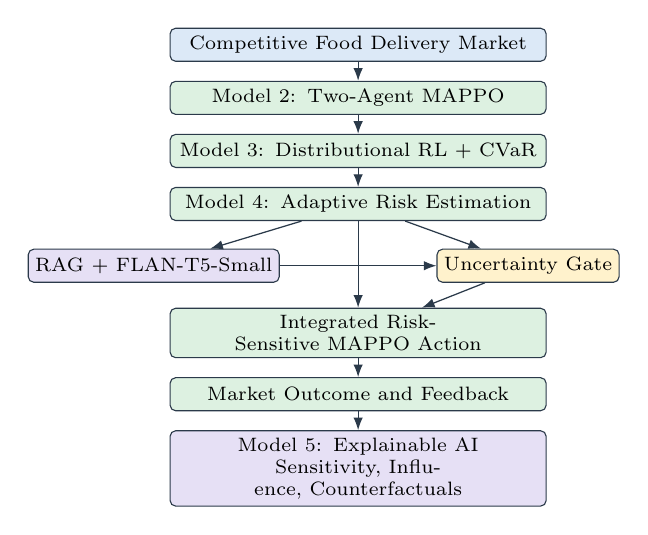
\begin{tikzpicture}[node distance=2.4mm and 2mm]
  \node[inb, text width=46mm] (mk) {Competitive Food Delivery Market};
  \node[prc, text width=46mm, below=of mk] (m2) {Model 2: Two-Agent MAPPO};
  \node[prc, text width=46mm, below=of m2] (m3) {Model 3: Distributional RL + CVaR};
  \node[prc, text width=46mm, below=of m3] (m4) {Model 4: Adaptive Risk Estimation};
  \node[llm, below left=3.5mm and -14mm of m4] (rg) {RAG + FLAN-T5-Small};
  \node[gat, below right=3.5mm and -14mm of m4] (ug) {Uncertainty Gate};
  \node[prc, text width=46mm, below=11mm of m4] (ac) {Integrated Risk-Sensitive MAPPO Action};
  \node[prc, text width=46mm, below=of ac] (fb) {Market Outcome and Feedback};
  \node[llm, text width=46mm, below=of fb] (m5) {Model 5: Explainable AI\\ Sensitivity, Influence, Counterfactuals};
  \foreach \a/\b in {mk/m2,m2/m3,m3/m4,m4/ac,ac/fb} \draw[arr] (\a) -- (\b);
  \draw[arr] (m4) -- (rg); \draw[arr] (m4) -- (ug);
  \draw[arr] (rg) -- (ug);
  \draw[arr] (ug) -- (ac);
  \draw[arr, dashed] (fb) -- (m5);
\end{tikzpicture}
\caption{Complete integrated research architecture. Model 5 analyses the frozen integrated policy.}
\label{fig:full}
\end{figure}

\subsection{Evolution Across the Five Models}
The research system develops through the progression summarised in Table~\ref{tab:evo}.

\begin{table}[!t]
\centering
\caption{Evolution of the research framework.}
\label{tab:evo}
\small
\renewcommand{\arraystretch}{1.1}
\begin{tabularx}{\columnwidth}{c>{\raggedright\arraybackslash}p{24mm}>{\raggedright\arraybackslash}X}
\toprule
\textbf{Model} & \textbf{Primary Capability} & \textbf{Contribution} \\
\midrule
1 & Market simulation & Establishes the competitive delivery environment. \\
2 & MAPPO & Introduces learning-based multi-agent decisions. \\
3 & Distributional RL and CVaR & Introduces explicit downside-risk awareness. \\
4 & Adaptive risk and LLM/RAG & Adds stress-responsive risk and selective contextual guidance. \\
5 & Explainable AI & Measures and validates the behaviour of the integrated policy. \\
\bottomrule
\end{tabularx}
\end{table}

\subsection{Principal Integrated Achievements}
The completed system demonstrates the following capabilities:
\begin{enumerate}
  \item A repeatable competitive market simulator supporting sequential multi-agent decisions.
  \item A two-agent MAPPO learning framework with a common 14-dimensional observation and 25-action decision structure.
  \item Distributional return estimation using 25 quantiles and a CVaR-based risk mechanism.
  \item Adaptive risk estimation that responds to genuine environmental stress.
  \item Selective LLM guidance through RAG, contrastive action scoring, and a confidence gate.
  \item Quantitative explanation analysis using 8,064 normal and genuine-shock decision records.
  \item Feature-faithfulness evidence showing substantially stronger policy sensitivity for highly ranked features.
\end{enumerate}

% ================================================================= 9
\section{Consolidated Experimental Findings}

\subsection{Model-Wise Findings}
The contributions of the completed models are summarised in Table~\ref{tab:summary}.

\begin{table}[!t]
\centering
\caption{Summary of completed model contributions.}
\label{tab:summary}
\small
\renewcommand{\arraystretch}{1.1}
\begin{tabularx}{\columnwidth}{c>{\raggedright\arraybackslash}p{30mm}>{\raggedright\arraybackslash}X}
\toprule
\textbf{Model} & \textbf{Implemented Method} & \textbf{Reported Outcome} \\
\midrule
1 & Stochastic competitive market simulation & Repeatable environment with detailed operational records. \\
2 & Two-agent MAPPO & Trainable competitive decision policy and reusable checkpoint. \\
3 & Distributional critic and CVaR constraints & Improved reported fulfilment and lower tail-risk measure. \\
4 & Adaptive risk, RAG, FLAN-T5-Small and confidence gating & Higher profit and fulfilment, with lower tail CVaR than the adaptive control in both tested conditions. \\
5 & Feature sensitivity, LLM influence and counterfactual XAI & Quantitative explanation-faithfulness evidence across 8,064 decisions. \\
\bottomrule
\end{tabularx}
\end{table}

\subsection{Model 4 Performance Improvements}
The integrated Model 4 system achieved the improvements in Table~\ref{tab:improve} relative to the adaptive-risk-only control.

\begin{table}[!t]
\centering
\caption{Percentage and percentage-point improvements.}
\label{tab:improve}
\small
\begin{tabular}{lcc}
\toprule
\textbf{Metric} & \textbf{Normal} & \textbf{Genuine Shock} \\
\midrule
Profit per hour     & +3.22\%  & +4.46\% \\
Fulfilment          & +2.71 pp & +3.00 pp \\
Tail CVaR reduction & 11.75\%  & 9.53\% \\
\bottomrule
\end{tabular}
\end{table}

\subsection{Explainability Improvements}
The feature-faithfulness experiments demonstrated the following top-to-bottom sensitivity ratios:
\begin{itemize}
  \item Normal condition: 7.38 times greater action-flip ratio.
  \item Genuine-shock condition: 8.86 times greater action-flip ratio.
  \item Normal condition: 20.33 times greater decision-margin-change ratio.
  \item Genuine-shock condition: 21.21 times greater decision-margin-change ratio.
\end{itemize}
These results provide quantitative evidence that the feature-ranking mechanism identifies variables with stronger influence on the actual policy.

% ================================================================= 10
\section{Conclusion}
This research developed a five-stage multi-agent decision-making framework for competitive food delivery platforms. The work began with the construction of a programmable market simulator that represents stochastic demand, competition, courier capacity, customer fulfilment, service delays, and operational outcomes. A two-agent MAPPO framework was then introduced to learn sequential pricing and incentive decisions.

The next stage incorporated distributional reinforcement learning and CVaR-based risk constraints, allowing the policy to represent return uncertainty and explicitly consider adverse outcomes. The integrated Model 4 system extended this framework through adaptive risk estimation and selective contextual guidance using RAG and FLAN-T5-Small. The confidence-gated integration ensured that the language model provided an additional action prior while MAPPO continued to determine the final action. The reported normal and genuine-shock evaluations demonstrated improvements in profitability, fulfilment, and the tail-risk measure relative to the adaptive-risk-only control.

Finally, Model 5 introduced a quantitative explainability framework for the frozen integrated policy. Using 8,064 decision records, the analysis examined feature sensitivity, LLM influence, counterfactual action changes, and explanation faithfulness. The resulting feature-faithfulness ratios demonstrated that highly ranked features produced substantially larger policy changes than low-ranked features.

Overall, the research establishes a connected framework that progresses from market simulation to competitive multi-agent learning, downside-risk control, adaptive contextual guidance, and quantitative explainability. The first complete integrated research model therefore combines:
\begin{equation*}
\begin{aligned}
&\text{Market Simulation} \rightarrow \text{MAPPO} \rightarrow \text{Distributional RL + CVaR}\\
&\rightarrow \text{Adaptive Risk + LLM/RAG} \rightarrow \text{Explainable AI}.
\end{aligned}
\end{equation*}

% ================================================================= REFERENCES
\begin{thebibliography}{25}

\bibitem{schulman2017ppo}
J.~Schulman, F.~Wolski, P.~Dhariwal, A.~Radford, and O.~Klimov, ``Proximal policy optimization algorithms,'' \emph{arXiv preprint arXiv:1707.06347}, 2017.

\bibitem{yu2022mappo}
C.~Yu \emph{et al.}, ``The surprising effectiveness of PPO in cooperative multi-agent games,'' in \emph{Advances in Neural Information Processing Systems}, 2022.

\bibitem{bellemare2017distributional}
M.~G. Bellemare, W.~Dabney, and R.~Munos, ``A distributional perspective on reinforcement learning,'' in \emph{Proc. Int. Conf. Machine Learning}, 2017.

\bibitem{dabney2018qr}
W.~Dabney, M.~Rowland, M.~G. Bellemare, and R.~Munos, ``Distributional reinforcement learning with quantile regression,'' in \emph{Proc. AAAI Conf. Artificial Intelligence}, 2018.

\bibitem{rockafellar2000cvar}
R.~T. Rockafellar and S.~Uryasev, ``Optimization of conditional value-at-risk,'' \emph{Journal of Risk}, vol.~2, pp.~21--41, 2000.

\bibitem{chow2014cvar}
Y.~Chow and M.~Ghavamzadeh, ``Algorithms for CVaR optimization in MDPs,'' in \emph{Advances in Neural Information Processing Systems}, vol.~27, 2014.

\bibitem{lewis2020rag}
P.~Lewis \emph{et al.}, ``Retrieval-augmented generation for knowledge-intensive NLP tasks,'' in \emph{Advances in Neural Information Processing Systems}, 2020.

\bibitem{chung2024flan}
H.~W. Chung \emph{et al.}, ``Scaling instruction-finetuned language models,'' \emph{Journal of Machine Learning Research}, vol.~25, 2024.

\bibitem{sundararajan2017ig}
M.~Sundararajan, A.~Taly, and Q.~Yan, ``Axiomatic attribution for deep networks,'' in \emph{Proc. Int. Conf. Machine Learning}, 2017.

\bibitem{deliverycenter}
Delivery Center, ``Food and goods orders in Brazil,'' Kaggle dataset. [Online]. Available: \url{https://www.kaggle.com/datasets/nosbielcs/brazilian-delivery-center}

\bibitem{zomato}
H.~P. Himanshu, ``Zomato Bangalore restaurants,'' Kaggle dataset. [Online]. Available: \url{https://www.kaggle.com/datasets/himanshupoddar/zomato-bangalore-restaurants}

\bibitem{flant5small}
Google Research, ``FLAN-T5-Small,'' Hugging Face Model Repository. [Online]. Available: \url{https://huggingface.co/google/flan-t5-small}

\bibitem{lowe2017maddpg}
R.~Lowe, Y.~Wu, A.~Tamar, J.~Harb, P.~Abbeel, and I.~Mordatch, ``Multi-agent actor-critic for mixed cooperative-competitive environments,'' in \emph{Advances in Neural Information Processing Systems}, vol.~30, 2017.

\bibitem{schulman2016gae}
J.~Schulman, P.~Moritz, S.~Levine, M.~Jordan, and P.~Abbeel, ``High-dimensional continuous control using generalized advantage estimation,'' in \emph{Proc. Int. Conf. Learning Representations}, 2016.

\bibitem{lin2018fleet}
K.~Lin, R.~Zhao, Z.~Xu, and J.~Zhou, ``Efficient large-scale fleet management via multi-agent deep reinforcement learning,'' in \emph{Proc. ACM SIGKDD Int. Conf. Knowledge Discovery \& Data Mining}, 2018, pp.~1774--1783.

\bibitem{li2019meanfield}
M.~Li, Z.~Qin, Y.~Jiao, Y.~Yang, J.~Wang, C.~Wang, G.~Wu, and J.~Ye, ``Efficient ridesharing order dispatching with mean field multi-agent reinforcement learning,'' in \emph{Proc. World Wide Web Conf.}, 2019, pp.~983--994.

\bibitem{dabney2018iqn}
W.~Dabney, G.~Ostrovski, D.~Silver, and R.~Munos, ``Implicit quantile networks for distributional reinforcement learning,'' in \emph{Proc. Int. Conf. Machine Learning}, 2018, pp.~1096--1105.

\bibitem{tamar2015cvar}
A.~Tamar, Y.~Glassner, and S.~Mannor, ``Optimizing the CVaR via sampling,'' in \emph{Proc. AAAI Conf. Artificial Intelligence}, 2015.

\bibitem{tessler2019rcpo}
C.~Tessler, D.~J. Mankowitz, and S.~Mannor, ``Reward constrained policy optimization,'' in \emph{Proc. Int. Conf. Learning Representations}, 2019.

\bibitem{garcia2015safe}
J.~Garc\'ia and F.~Fern\'andez, ``A comprehensive survey on safe reinforcement learning,'' \emph{Journal of Machine Learning Research}, vol.~16, no.~1, pp.~1437--1480, 2015.

\bibitem{raffel2020t5}
C.~Raffel \emph{et al.}, ``Exploring the limits of transfer learning with a unified text-to-text transformer,'' \emph{Journal of Machine Learning Research}, vol.~21, no.~140, pp.~1--67, 2020.

\bibitem{ribeiro2016lime}
M.~T. Ribeiro, S.~Singh, and C.~Guestrin, ``\,`Why should I trust you?': Explaining the predictions of any classifier,'' in \emph{Proc. ACM SIGKDD Int. Conf. Knowledge Discovery \& Data Mining}, 2016, pp.~1135--1144.

\bibitem{lundberg2017shap}
S.~M. Lundberg and S.-I. Lee, ``A unified approach to interpreting model predictions,'' in \emph{Advances in Neural Information Processing Systems}, vol.~30, 2017.

\bibitem{wachter2018counterfactual}
S.~Wachter, B.~Mittelstadt, and C.~Russell, ``Counterfactual explanations without opening the black box: Automated decisions and the GDPR,'' \emph{Harvard Journal of Law \& Technology}, vol.~31, no.~2, pp.~841--887, 2018.

\bibitem{hooker2019roar}
S.~Hooker, D.~Erhan, P.-J. Kindermans, and B.~Kim, ``A benchmark for interpretability methods in deep neural networks,'' in \emph{Advances in Neural Information Processing Systems}, vol.~32, 2019.

\end{thebibliography}

\end{document}
